% 第4章第1节：向量的表示（坐标向量、相等、零向量与标准坐标向量、标量）、向量的运算（加法与数乘、线性组合、内积、长度与距离、范数）、向量运算的性质（加法与数乘的性质、内积的性质、范数的性质）。夹角与Cauchy--Schwarz不等式见第5章内积空间一节。

\section{向量}
\label{sec:ls-vectors}
\label{sec:ls-objects}
\label{sec:linear-algebra-objects}
\label{sec:linear-algebra-space-representations}
\label{sec:prelim-vectors-matrices}

三次观测的输入与输出各是一串数；两个模型各给出一串预测，需要合并或比较；预测减去观测又是一串误差，需要判断它有多大。这些问题处理的都是按固定次序排列的一串实数，也就是向量。本节先规定向量怎样书写、何时相等；再定义向量之间的运算，回答怎样把几串数合并成一串、怎样把两串数配成一个数、怎样用一个数衡量一串数的大小；最后按运算整理它们满足的规则与不等式。

\subsection{向量的表示}
\label{sec:ls-vector-representation}
\label{sec:prelim-vector-records}

用一串数记录数据之前，须先说清这串数怎样排列、每个位置记录什么、两串数何时算作相同。

\paragraph{坐标向量}
第~\ref{sec:sets-power-sets-products}节把$\mathbb R^d$定义为全部有序$d$元实数组的集合。把其中一个元素的$d$个实数按原有次序竖排成一列，得到实坐标向量（real coordinate vector）：
\[
 \bm u=\begin{pmatrix}u_1\\\vdots\\u_d\end{pmatrix}\in\mathbb R^d,
\]
其中$u_j$是第$j$个坐标，$d$是维数。定位向量中的一个数只需要一个索引$j$。

本书默认使用这样的列向量；把同样的数横排成一行，称为行向量。上标$\top$表示\term{转置}（transpose），它把行向量改写成列向量，也把列向量改写成行向量。因此$(u_1,\ldots,u_d)^\top$就是上面的列向量，正文中常用这种写法节省篇幅。

用向量记录数据时，每个位置的含义须预先固定。例如三次观测的（输入，输出）依次为$(1,0)$、$(2,4)$、$(3,6)$，把输入和输出分别排成向量，得到
\[
 \bm x=\begin{pmatrix}1\\2\\3\end{pmatrix},\qquad
 \bm y=\begin{pmatrix}0\\4\\6\end{pmatrix}.
\]
$\bm x$记录输入，$\bm y$记录观测输出；两个向量的第$i$个位置对应同一次观测。正因为位置的含义一致，后面才能把两个向量逐位置地相加、相乘。

\paragraph{相等、零向量与标准坐标向量}
两个向量相等，要求维数相同且对应坐标分别相等。次序是向量的一部分，因此$(1,2)^\top\neq(2,1)^\top$：两者含有同样的两个数，第一个坐标却不同。

所有坐标都为零的向量称为零向量，记作$\bm0$。第$j$个坐标为$1$、其余坐标为$0$的向量记作$\bm e_j$，$\bm e_1,\ldots,\bm e_d$称为$\mathbb R^d$的标准坐标向量；每个$\bm e_j$只“点亮”第$j$个位置。例如在$\mathbb R^3$中，$\bm e_2=(0,1,0)^\top$。

\paragraph{标量}
\phantomsection
\label{sec:ls-scalars}
与向量相对，单个实数称为标量（scalar）。它在向量运算中有两种身份。一种是被记录的结果，例如拟合值$y_i$、误差$e_i$，它们各是某个向量的一个坐标。另一种是缩放其他对象的系数，例如下一小节线性组合$\sum_j c_j\bm v_j$中的$c_j$，它表示向量$\bm v_j$在组合中占多少份。标量只是一个数，没有需要索引的位置。本书的向量坐标与系数都取实数。

\subsection{向量的运算}
\label{sec:ls-vector-operations}

两个预测分支各给出一列输出，怎样合并成一列？两列数之间能否算出一个数，表示它们“配合”得怎样？一列误差又该算多大？本小节依次定义回答这些问题的运算：加法与数乘逐位置进行，二者结合得到线性组合；内积把两个向量配成一个数；长度和更一般的范数用一个非负数衡量向量的大小。这些运算满足的规则放在下一小节。

\subsubsection{加法与数乘}
\phantomsection
\label{sec:ls-addition-scaling}

同维向量按对应坐标相加减；实数$c$与向量的数乘（scalar multiplication）把每个坐标乘以同一个$c$。对$\bm x,\bm y\in\mathbb R^d$与$c\in\mathbb R$，
\[
 (\bm x+\bm y)_j=x_j+y_j,\qquad
 (\bm x-\bm y)_j=x_j-y_j,\qquad
 (c\bm x)_j=cx_j,\qquad j=1,\ldots,d.
\]
特别地，$0\bm x=\bm0$；$-\bm x=(-1)\bm x$称为$\bm x$的相反向量。两种运算都不让不同位置的数相互影响：结果的第$j$个坐标只由输入的第$j$个坐标决定，结果仍是$d$维向量。

下面按定义逐坐标计算一组二维向量的加法、减法与数乘。
\begin{example}[向量的加法、减法与数乘]
\label{ex:ls-vector-addition-scaling}
给定：$\bm x=(1,2)^\top$，$\bm y=(3,-1)^\top$，$\bm z=(1,-3)^\top$，$c=2$。
计算：逐坐标相加、相减与相乘，
\[
 \begin{aligned}
 \bm x+\bm y&=\begin{pmatrix}1+3\\2+(-1)\end{pmatrix}=\begin{pmatrix}4\\1\end{pmatrix},\qquad
 \bm x-\bm y=\begin{pmatrix}1-3\\2-(-1)\end{pmatrix}=\begin{pmatrix}-2\\3\end{pmatrix},\\
 c\bm z&=\begin{pmatrix}2\cdot1\\2\cdot(-3)\end{pmatrix}=\begin{pmatrix}2\\-6\end{pmatrix}.
 \end{aligned}
\]
结论：三个结果都是二维向量，每个坐标只用到输入在同一位置上的坐标。
\end{example}

两个向量能够相加，要求维数相同，并且对应位置的含义相同。维数不同的向量无法逐位置配对，加法没有定义。维数相同而位置含义不同时，逐坐标相加虽然算得出数，结果却没有意义，下面的反例说明这一点。
\begin{example}[反例：维数相同而位置含义不同]
\label{ex:ls-mismatched-positions}
给定：$\bm u=(h_1,w_1)^\top$按“身高、体重”的次序记录第一个人，$\bm v=(w_2,h_2)^\top$按“体重、身高”的次序记录第二个人，两者都属于$\mathbb R^2$。
计算：按定义，$\bm u+\bm v=(h_1+w_2,\ w_1+h_2)^\top$。
结论：结果的第一个坐标是一个人的身高加另一个人的体重，不表示任何有意义的量。加法在形式上有定义；只有先把$\bm v$改写成同样次序的$(h_2,w_2)^\top$，相加才有意义。
\end{example}

\subsubsection{线性组合}

若干同维向量分别乘以系数后相加，得到
\[
 c_1\bm v_1+c_2\bm v_2+\cdots+c_k\bm v_k=\sum_{j=1}^k c_j\bm v_j,
\]
称为$\bm v_1,\ldots,\bm v_k$的一个\term{线性组合}（linear combination），$c_1,\ldots,c_k$称为系数。结果的第$i$个坐标是$\sum_jc_j(\bm v_j)_i$，即各向量在该位置的坐标按同一组系数作的加权和。系数是实数，不要求非负，也不要求和为$1$。

线性组合可以一次写出一组预测及其误差。下面回到前面的观测向量。
\begin{example}[残差向量是线性组合]
\label{ex:ls-residual-vector}
给定：观测向量$\bm x=(1,2,3)^\top$与$\bm y=(0,4,6)^\top$，以及用输入的$w$倍预测输出的规则。
计算：三次预测合起来是$w\bm x$。预测减观测得到残差向量（residual vector）
\[
 \bm r=w\bm x-\bm y=w\bm x+(-1)\bm y,
\]
它是$\bm x,\bm y$以$w$和$-1$为系数的线性组合。取$w=1$，
\[
 \bm r=\begin{pmatrix}1-0\\2-4\\3-6\end{pmatrix}=\begin{pmatrix}1\\-2\\-3\end{pmatrix}.
\]
结论：残差向量的第$i$个坐标是第$i$次观测的预测误差，三个误差由同一组系数一次写出。
\end{example}

下面这个例子将贯穿整个线性空间部分。它用线性组合说明，两个特征的取值向量可以只相差一个很短的向量。
\begin{example}[贯穿例：两个几乎相同的特征]
\label{ex:ls-nearly-collinear-features}
给定：三个样本的两个特征分别取值
\begin{equation*}
 \bm c_1=\begin{pmatrix}1\\1\\1\end{pmatrix},\qquad
 \bm c_2=\begin{pmatrix}1\\1+\varepsilon\\1-\varepsilon\end{pmatrix},\qquad
 \bm q=\begin{pmatrix}0\\1\\-1\end{pmatrix},
\end{equation*}
其中$\bm c_1$、$\bm c_2$分别是第一、第二个特征的取值向量，$\varepsilon$是一个实参数。
验证：第一个特征在三个样本上都取$1$；第二个特征在第一个样本上也取$1$，在第二、三个样本上分别取$1+\varepsilon$与$1-\varepsilon$。逐坐标计算，
\[
 \bm c_1+\varepsilon\bm q=\begin{pmatrix}1+0\\1+\varepsilon\\1-\varepsilon\end{pmatrix}=\bm c_2.
\]
结论：$\bm c_2=\bm c_1+\varepsilon\bm q$，即第二个特征的取值向量是$\bm c_1$与$\bm q$以$1$和$\varepsilon$为系数的线性组合。$|\varepsilon|$很小时，$\bm c_1$与$\bm c_2$几乎是同一串数。
\end{example}
两列的方向“几乎相同”究竟指什么，要等第~\ref{sec:ls-inner-product-definition}节用内积定义了夹角才能说清。

\subsubsection{内积}
\phantomsection
\label{sec:ls-inner-products}
\label{sec:prelim-vector-inner-length}

线性预测对一次观测的输入$x_1,\ldots,x_d$和一组权重$w_1,\ldots,w_d$计算加权和$\sum_jx_jw_j$：两串数逐项相乘再相加。把这种运算单独定义出来：对$\bm x,\bm y\in\mathbb R^d$，标准坐标下的欧氏内积为
\[
 \langle\bm x,\bm y\rangle
 =\sum_{j=1}^d x_jy_j,
\]
也写作$\bm x^\top\bm y$。输入是两个同维向量，输出是一个标量。矩阵一节将看到，$\bm x^\top\bm y$正是$1\times d$矩阵与$d\times1$矩阵的乘积。

内积为零的情形有专门的名称：$\langle\bm x,\bm y\rangle=0$时称两向量\term{正交}（orthogonal）。下面先计算一个内积，再检查平面上两对向量是否正交。
\begin{example}[内积与正交的计算]
\label{ex:ls-inner-product-orthogonality}
给定：$\mathbb R^2$中的三对向量：$(2,-1)^\top$与$(3,4)^\top$；标准坐标向量$\bm e_1=(1,0)^\top$与$\bm e_2=(0,1)^\top$；$(1,1)^\top$与$(1,-1)^\top$。
计算：按定义逐项相乘再相加，
\[
 \begin{gathered}
 \left\langle\begin{pmatrix}2\\-1\end{pmatrix},\begin{pmatrix}3\\4\end{pmatrix}\right\rangle=2\cdot3+(-1)\cdot4=2,\\
 \langle\bm e_1,\bm e_2\rangle=1\cdot0+0\cdot1=0,\qquad
 \left\langle\begin{pmatrix}1\\1\end{pmatrix},\begin{pmatrix}1\\-1\end{pmatrix}\right\rangle=1\cdot1+1\cdot(-1)=0.
 \end{gathered}
\]
结论：第一对向量不正交；后两对向量正交，在平面上它们正是两对互相垂直的方向。
\end{example}
在一般维数下，正交为什么可以称为“垂直”，要等第~\ref{sec:ls-inner-product-definition}节用内积定义了夹角才能说明。

\paragraph{内积的公理}
欧氏内积满足对称性、双线性与正定性三条性质，第~\ref{sec:ls-vector-operation-properties}节将逐条验证。后面由内积导出的长度、夹角等结论只用到这三条，不用到逐项相乘的具体公式。所以把它们取作内积的公理：凡满足这三条的配对都称为内积，都可以像欧氏内积一样使用。
\begin{definition}[实内积]
\label{def:linear-algebra-inner-product}
$\mathbb R^d$上的\term{内积}（inner product）是映射$\langle\cdot,\cdot\rangle:\mathbb R^d\times\mathbb R^d\to\mathbb R$，同时满足下列三条公理。
\begin{enumerate}
 \item 双线性：对两个变量分别保持线性组合，即$\langle a\bm x+b\bm y,\bm z\rangle=a\langle\bm x,\bm z\rangle+b\langle\bm y,\bm z\rangle$，且对第二变量同样线性。
 \item 对称性：$\langle\bm x,\bm y\rangle=\langle\bm y,\bm x\rangle$。
 \item 正定性：$\langle\bm x,\bm x\rangle>0$对所有非零$\bm x$成立，且$\langle\bm x,\bm x\rangle=0$当且仅当$\bm x=\bm0$。
\end{enumerate}
\end{definition}
任一内积都可以像欧氏内积一样定义长度，见下一小节。公理只用到加法与数乘，因此同形矩阵上也可以按同样的三条规定内积，矩阵一节的Frobenius内积就是一例；第~\ref{sec:ls-inner-product-spaces}节将在更一般的对象上这样做。

\subsubsection{长度与距离}
\phantomsection
\label{sec:linear-algebra-length-angle-distance}

向量与自身的内积$\langle\bm x,\bm x\rangle=\sum_jx_j^2$是各坐标的平方和，因而非负，可以开平方。开平方后得到向量的长度
\begin{equation}
 \lVert\bm x\rVert=\sqrt{\langle\bm x,\bm x\rangle}.
 \label{eq:linear-algebra-inner-product-norm}
\end{equation}
标准内积给出的长度称为欧氏范数（Euclidean norm）或$2$范数，记作
\[
 \lVert\bm x\rVert_2=\sqrt{\sum_{j=1}^d x_j^2},
\]
它把平面上的勾股定理推广到$d$个坐标。

长度为$1$的向量称为单位向量。非零向量$\bm x$除以自身长度，得到的$\bm x/\lVert\bm x\rVert_2$各坐标平方和为$1$，是一个单位向量；它与$\bm x$方向相同，只是去掉了大小。

$\bm x$与$\bm y$的欧氏距离定义为差向量的长度$\lVert\bm x-\bm y\rVert_2$。下面计算前面残差向量的长度，以及平面上两点的距离。
\begin{example}[长度与距离的计算]
\label{ex:ls-length-distance}
给定：示例~\ref{ex:ls-residual-vector}中$w=1$时的残差$\bm r=(1,-2,-3)^\top$；平面上的两点$(1,2)^\top$与$(4,6)^\top$。
计算：
\[
 \begin{gathered}
 \lVert\bm r\rVert_2^2=1^2+(-2)^2+(-3)^2=14,\\
 \left\lVert\begin{pmatrix}1\\2\end{pmatrix}-\begin{pmatrix}4\\6\end{pmatrix}\right\rVert_2=\sqrt{(-3)^2+(-4)^2}=5.
 \end{gathered}
\]
结论：$\lVert\bm r\rVert_2^2=14$正是$w=1$时三次观测的平方误差总和；两点之间的欧氏距离为$5$。
\end{example}
用距离比较实际数值记录时，应先约定各坐标的单位和尺度，否则数值大的坐标会支配距离。

\subsubsection{范数}

欧氏长度只是衡量大小的一种口径。同一个误差向量$(1,1)^\top$，按绝对偏差之和计为$2$，按欧氏长度计为$\sqrt2$，只看最大坐标偏差则计为$1$。不同任务看重的误差含义不同。但无论采用哪种口径，大小都应当满足几条共同要求：零向量大小为零，非零向量大小为正；整体放大$c$倍，大小放大$|c|$倍；两段误差相加，总大小不超过各自大小之和。把这些要求写成公理，就得到范数。
\begin{definition}[范数]
\label{def:functional-normed-space}
映射$\lVert\cdot\rVert:\mathbb R^d\to[0,\infty)$若对任意$\bm x,\bm y\in\mathbb R^d$与$c\in\mathbb R$满足下列四条，就称为$\mathbb R^d$上的\term{范数}（norm）。它给出距离$\lVert\bm x-\bm y\rVert$。
\begin{enumerate}
 \item 非负性：$\lVert\bm x\rVert\geq0$。
 \item 正定性：$\lVert\bm x\rVert=0$当且仅当$\bm x=\bm0$。
 \item 齐次性：$\lVert c\bm x\rVert=|c|\,\lVert\bm x\rVert$。
 \item 三角不等式：$\lVert\bm x+\bm y\rVert\leq\lVert\bm x\rVert+\lVert\bm y\rVert$。
\end{enumerate}
\end{definition}
四条要求只用到加法与数乘，下一节对同形矩阵规定范数时沿用同样的四条。

范数给出的距离同样满足三角不等式。由$(\bm x-\bm z)+(\bm z-\bm y)=\bm x-\bm y$，把范数的三角不等式用于$\bm x-\bm z$与$\bm z-\bm y$，得到
\[
 \lVert\bm x-\bm y\rVert\leq\lVert\bm x-\bm z\rVert+\lVert\bm z-\bm y\rVert,
\]
即经由第三个点绕行，不会比直接相连更短。

有限坐标中最常用的是$p$范数：
\[
 \lVert\bm x\rVert_p=\left(\sum_j|x_j|^p\right)^{1/p}\quad(1\leq p<\infty),
 \qquad
 \lVert\bm x\rVert_\infty=\max_j|x_j|.
\]
$p=1$累加绝对偏差；$p=2$累计平方偏差再开方，就是欧氏长度；$p=\infty$取最大坐标偏差。下面在同一个向量上比较这三种口径。
\begin{example}[三种$p$范数的计算]
\label{ex:ls-p-norms}
给定：$\bm x=(3,-4)^\top$。
计算：
\[
 \begin{gathered}
 \lVert\bm x\rVert_1=|3|+|-4|=7,\qquad
 \lVert\bm x\rVert_2=\sqrt{3^2+(-4)^2}=5,\\
 \lVert\bm x\rVert_\infty=\max\{|3|,|-4|\}=4.
 \end{gathered}
\]
结论：同一个向量在三种口径下的大小依次为$7$、$5$、$4$，数值随口径而变。
\end{example}
$p$范数的非负性、正定性与齐次性可以直接从公式读出，三角不等式在下一小节证明。图~\ref{fig:ls-norm-unit-balls}比较三种口径下单位球$\{\bm x:\lVert\bm x\rVert\leq1\}$的形状。
\begin{figure*}[htbp]
  \centering
  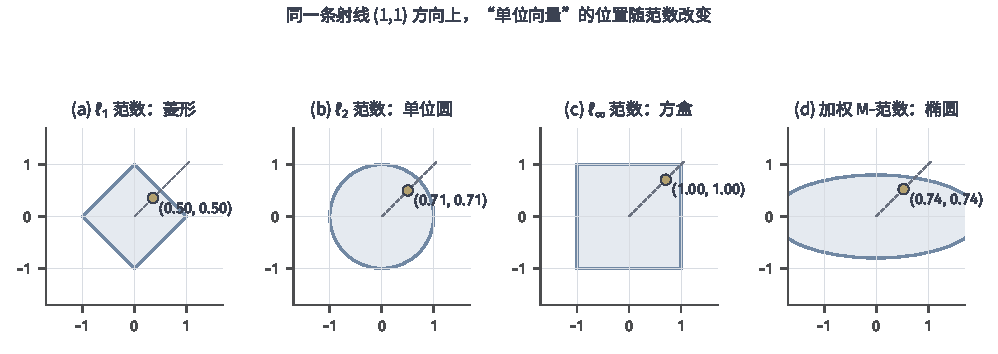
\includegraphics[width=169mm]{figures/01-mathematical-preliminaries-upper/03-linear-spaces/matplotlib/ls-norm-unit-balls/ls-norm-unit-balls.pdf}
  \caption{同一向量在不同范数下的“单位球”形状。左：$\ell_1$单位球为菱形（累加绝对偏差）；中：$\ell_2$单位球为圆（欧氏长度）；右：$\ell_\infty$单位球为正方形（最大坐标偏差）。同一个点$(1,1)$的范数依次为$2$、$\sqrt2$、$1$，单位球大小随口径而变，三者之间的倍数关系由正文的显式不等式给出。三图坐标尺度相同，为解析教学例。}
  \label{fig:ls-norm-unit-balls}
\end{figure*}

有时只关心向量的一部分信息，这时允许非零向量的大小为零，但保留齐次性与三角不等式。这样的尺度称为\term{半范数}（seminorm）。它给出的“距离”可能把不同的点判为距离为零，下面的例子说明这一点。
\begin{example}[只看第一个坐标的半范数]
\label{ex:ls-seminorm-first-coordinate}
给定：$\mathbb R^2$上的函数$p(\bm x)=|x_1|$。
验证：$p(\bm x)\geq0$；$p(c\bm x)=|cx_1|=|c|\,p(\bm x)$；$p(\bm x+\bm y)=|x_1+y_1|\leq|x_1|+|y_1|=p(\bm x)+p(\bm y)$。所以$p$满足非负性、齐次性与三角不等式。但非零向量$(0,1)^\top$满足$p\bigl((0,1)^\top\bigr)=0$，正定性不成立。
结论：$p$是半范数而不是范数。它判定$(0,0)^\top$与$(0,1)^\top$的距离为$p\bigl((0,-1)^\top\bigr)=0$，完全忽略了第二个坐标上的差别。
\end{example}
使用半范数之前，须先说明哪些差别被有意忽略。

\subsection{向量运算的性质}
\label{sec:ls-vector-operation-properties}

上一小节只给出了运算的定义；实际推导时还要知道哪些变形允许做、哪些估计一定成立。本小节按运算分组：先是加法与数乘的八条规则，再是内积的三条基本性质，最后是$p$范数满足的Hölder不等式与Minkowski不等式、欧氏范数特有的平行四边形恒等式，以及常用范数之间的比较。由内积公理推出的Cauchy--Schwarz不等式与夹角对一般内积都成立，放到第~\ref{sec:ls-inner-product-definition}节统一讨论。

\subsubsection{加法与数乘的性质}
\label{sec:ls-vector-operation-rules}

加法与数乘逐坐标定义，只用到实数的加法与乘法，所以下面每一条都可以在任一坐标上用实数运算直接验证。设$\bm u,\bm v,\bm w\in\mathbb R^d$，$a,b\in\mathbb R$。

\paragraph{加法交换律与结合律}
\[
 \bm u+\bm v=\bm v+\bm u,\qquad
 (\bm u+\bm v)+\bm w=\bm u+(\bm v+\bm w).
\]

\paragraph{零向量与相反向量}
\[
 \bm u+\bm0=\bm u,\qquad
 \bm u+(-\bm u)=\bm0.
\]

\paragraph{数乘结合律与单位数}
\[
 a(b\bm u)=(ab)\bm u,\qquad
 1\bm u=\bm u.
\]

\paragraph{分配律}
\[
 (a+b)\bm u=a\bm u+b\bm u,\qquad
 a(\bm u+\bm v)=a\bm u+a\bm v.
\]

有了这八条规则，有限次加法与数乘可以任意添加括号、交换加项次序并展开，结果不变，所以线性组合可以像多项式一样合并同类项。下一节的同形矩阵、再后面的多维数组也逐项相加与数乘，同样的验证对它们逐字成立。第~\ref{chap:linear-representation}章将看到，后面许多结论只依赖这八条规则，而不依赖对象是一列数还是一张表。

\subsubsection{内积的性质}

下面逐条验证欧氏内积满足定义~\ref{def:linear-algebra-inner-product}的三条公理。设$\bm x,\bm y,\bm z\in\mathbb R^d$，$a,b\in\mathbb R$。

\paragraph{对称性}
\[
 \langle\bm x,\bm y\rangle=\langle\bm y,\bm x\rangle,
\]
因为每一项$x_jy_j=y_jx_j$。

\paragraph{双线性}
\[
 \langle a\bm x+b\bm z,\bm y\rangle=a\langle\bm x,\bm y\rangle+b\langle\bm z,\bm y\rangle,
\]
由有限和的运算法则$\sum_j(ax_j+bz_j)y_j=a\sum_jx_jy_j+b\sum_jz_jy_j$得到；再由对称性，对第二个变量同样成立。

\paragraph{正定性}
\[
 \langle\bm x,\bm x\rangle\geq0,\qquad
 \langle\bm x,\bm x\rangle=0\iff\bm x=\bm0,
\]
因为$\langle\bm x,\bm x\rangle=\sum_jx_j^2$，而非负数之和为零时每一项都为零。

\subsubsection{范数的性质}
\label{sec:ls-norms-distances}
\label{sec:linear-algebra-distance-relations}

上一小节的$p$范数满足非负性、正定性与齐次性，这可以直接从公式读出；需要证明的是三角不等式。$p=1$时，对每个坐标用实数的$|x_j+y_j|\leq|x_j|+|y_j|$再求和即得；$p=\infty$时，同一不等式给出$|x_j+y_j|\leq\lVert\bm x\rVert_\infty+\lVert\bm y\rVert_\infty$，再对$j$取最大值即得。$1<p<\infty$时，先要建立下面的不等式，它用一对互相配合的$p$范数与$q$范数控制两个向量逐项乘积之和。

\paragraph{Hölder不等式}
\begin{theorem}[有限维Hölder不等式]
\label{thm:linear-algebra-holder}
设$1\leq p,q\leq\infty$且$1/p+1/q=1$（约定$1/\infty=0$），则$|\bm x^\top\bm y|\leq\lVert\bm x\rVert_p\lVert\bm y\rVert_q$。
\end{theorem}
\begin{proof}
先设$1<p,q<\infty$，分三步证明。

第一步，证明Young不等式：对$u,v\geq0$，
\[
 uv\leq\frac{u^p}{p}+\frac{v^q}{q}.
\]
$u=0$时左侧为零，不等式成立。$u>0$时令$t=v/u^{p-1}\geq0$。由$1/p+1/q=1$得$(p-1)q=p$，于是$v^q=t^qu^p$、$uv=tu^p$，不等式化为
\[
 u^p\Bigl(\frac1p+\frac{t^q}{q}-t\Bigr)\geq0.
\]
函数$f(t)=1/p+t^q/q-t$的导数$t^{q-1}-1$在$0<t<1$时为负、在$t>1$时为正，所以$f$在$t\geq0$上的最小值是$f(1)=1/p+1/q-1=0$，不等式成立。

第二步，在单位尺度下求和。若$\bm x$或$\bm y$为零向量，结论两侧都为零。否则令$u_j=|x_j|/\lVert\bm x\rVert_p$、$v_j=|y_j|/\lVert\bm y\rVert_q$，则$\sum_ju_j^p=\sum_jv_j^q=1$。对每个$j$用Young不等式再求和，
\[
 \sum_ju_jv_j\leq\frac1p\sum_ju_j^p+\frac1q\sum_jv_j^q=\frac1p+\frac1q=1.
\]

第三步，恢复尺度。上式两边乘以$\lVert\bm x\rVert_p\lVert\bm y\rVert_q$，再用$|\bm x^\top\bm y|\leq\sum_j|x_j||y_j|$，即得
\[
 |\bm x^\top\bm y|\leq\sum_j|x_j||y_j|\leq\lVert\bm x\rVert_p\lVert\bm y\rVert_q.
\]

端点情形直接估计。$p=1$、$q=\infty$时，
\[
 \sum_j|x_j||y_j|\leq\Bigl(\max_j|y_j|\Bigr)\sum_j|x_j|=\lVert\bm x\rVert_1\lVert\bm y\rVert_\infty;
\]
$p=\infty$、$q=1$时交换两个向量的角色。
\end{proof}
$p=q=2$时，它给出$|\bm x^\top\bm y|\leq\lVert\bm x\rVert_2\lVert\bm y\rVert_2$。第~\ref{sec:ls-inner-product-definition}节将只用内积公理，对任一内积证明同样形式的不等式，即Cauchy--Schwarz不等式。

\paragraph{Minkowski不等式}
\[
 \lVert\bm x+\bm y\rVert_p\leq\lVert\bm x\rVert_p+\lVert\bm y\rVert_p,\qquad1\leq p\leq\infty.
\]
$p=1,\infty$的情形已在本小节开头说明。下面设$1<p<\infty$，并设$\bm x+\bm y\neq\bm0$（否则左侧为零）。取$q=p/(p-1)$，则$1/p+1/q=1$。先对每个坐标用实数的三角不等式，
\[
 |x_j+y_j|^p=|x_j+y_j|^{p-1}|x_j+y_j|\leq|x_j+y_j|^{p-1}|x_j|+|x_j+y_j|^{p-1}|y_j|.
\]
记$\bm s$为坐标$s_j=|x_j+y_j|^{p-1}$的向量。由$(p-1)q=p$，
\[
 \lVert\bm s\rVert_q=\Bigl(\sum_j|x_j+y_j|^{p}\Bigr)^{1/q}=\lVert\bm x+\bm y\rVert_p^{p/q}=\lVert\bm x+\bm y\rVert_p^{p-1}.
\]
把逐坐标的不等式对$j$求和，右侧两部分分别是$\bm s$与$(|x_1|,\ldots,|x_d|)^\top$、$\bm s$与$(|y_1|,\ldots,|y_d|)^\top$的内积，各用一次Hölder不等式，得到
\[
 \lVert\bm x+\bm y\rVert_p^p\leq\lVert\bm s\rVert_q\bigl(\lVert\bm x\rVert_p+\lVert\bm y\rVert_p\bigr)
 =\lVert\bm x+\bm y\rVert_p^{p-1}\bigl(\lVert\bm x\rVert_p+\lVert\bm y\rVert_p\bigr).
\]
两边除以$\lVert\bm x+\bm y\rVert_p^{p-1}>0$即得。于是每个$p$范数都满足范数的四条要求；取$p=2$，欧氏长度满足三角不等式。

\paragraph{平行四边形恒等式}
$p$范数都满足范数的四条要求，但欧氏范数还由标准内积给出，因而多满足一条一般范数未必满足的等式：
\begin{equation}
 \lVert\bm x+\bm y\rVert_2^2+\lVert\bm x-\bm y\rVert_2^2
 =2\lVert\bm x\rVert_2^2+2\lVert\bm y\rVert_2^2.
 \label{eq:functional-parallelogram-identity}
\end{equation}
它称为\term{平行四边形恒等式}。几何上，以$\bm x,\bm y$为邻边的平行四边形，两条对角线长度的平方和等于四条边长度的平方和。证明时按前面验证的内积双线性与对称性展开，
\[
 \lVert\bm x\pm\bm y\rVert_2^2=\langle\bm x\pm\bm y,\bm x\pm\bm y\rangle=\lVert\bm x\rVert_2^2\pm2\langle\bm x,\bm y\rangle+\lVert\bm y\rVert_2^2,
\]
两式相加，交叉项$\pm2\langle\bm x,\bm y\rangle$相互抵消，即得式~\eqref{eq:functional-parallelogram-identity}。

推导只用到两点：长度由内积按式~\eqref{eq:linear-algebra-inner-product-norm}给出，内积满足双线性与对称性。所以把标准内积换成定义~\ref{def:linear-algebra-inner-product}中的任一内积，它给出的长度同样满足这一恒等式。

反过来，恒等式可以检验一个范数是否来自内积：只要某个范数在一对向量上使恒等式两侧不等，它就不可能由任何内积给出。下面的反例用这个办法检验$\ell_1$与$\ell_\infty$范数。
\begin{example}[反例：$\ell_1$与$\ell_\infty$范数不来自内积]
\label{ex:ls-l1-linf-not-inner-product}
给定：$\mathbb R^2$中的$\bm x=\bm e_1$、$\bm y=\bm e_2$，于是$\bm x+\bm y=(1,1)^\top$，$\bm x-\bm y=(1,-1)^\top$。
计算：对$\ell_1$范数，
\[
 \lVert\bm x+\bm y\rVert_1^2+\lVert\bm x-\bm y\rVert_1^2=2^2+2^2=8,\qquad
 2\lVert\bm x\rVert_1^2+2\lVert\bm y\rVert_1^2=2\cdot1^2+2\cdot1^2=4;
\]
对$\ell_\infty$范数，
\[
 \lVert\bm x+\bm y\rVert_\infty^2+\lVert\bm x-\bm y\rVert_\infty^2=1^2+1^2=2,\qquad
 2\lVert\bm x\rVert_\infty^2+2\lVert\bm y\rVert_\infty^2=4.
\]
结论：两种范数都使恒等式两侧不等。所以不存在内积使$\lVert\bm x\rVert_1=\sqrt{\langle\bm x,\bm x\rangle}$对一切$\bm x$成立，$\ell_\infty$范数同样不是由内积给出的长度。
\end{example}

\paragraph{常用范数之间的比较}
对$\bm x\in\mathbb R^d$，
\[
 \lVert\bm x\rVert_\infty\leq\lVert\bm x\rVert_2\leq\sqrt d\,\lVert\bm x\rVert_\infty,
 \qquad
 \lVert\bm x\rVert_2\leq\lVert\bm x\rVert_1\leq\sqrt d\,\lVert\bm x\rVert_2.
\]
左端两式的依据是：平方和不小于其中最大的一项，所以$\lVert\bm x\rVert_\infty^2\leq\lVert\bm x\rVert_2^2$；展开$(\sum_j|x_j|)^2$时交叉项非负，所以$\lVert\bm x\rVert_1^2\geq\sum_jx_j^2=\lVert\bm x\rVert_2^2$。右端两式的依据是：$\sum_jx_j^2\leq d\max_jx_j^2$给出$\lVert\bm x\rVert_2\leq\sqrt d\,\lVert\bm x\rVert_\infty$；把$\sum_j|x_j|$看作$(|x_1|,\ldots,|x_d|)^\top$与全$1$向量的内积，用$p=q=2$的Hölder不等式，得到$\lVert\bm x\rVert_1\leq\sqrt d\,\lVert\bm x\rVert_2$。

下面在示例~\ref{ex:ls-p-norms}的向量上核对这四个不等式。
\begin{example}[范数比较的数值核对]
\label{ex:ls-norm-comparison-check}
给定：$d=2$，$\bm x=(3,-4)^\top$；由示例~\ref{ex:ls-p-norms}，$\lVert\bm x\rVert_1=7$，$\lVert\bm x\rVert_2=5$，$\lVert\bm x\rVert_\infty=4$。
验证：
\[
 4\leq5\leq4\sqrt2\approx5.66,\qquad
 5\leq7\leq5\sqrt2\approx7.07.
\]
结论：四个不等式都成立。右端的$\sqrt2$都不能换成$1$：$\lVert\bm x\rVert_2=5$大于$\lVert\bm x\rVert_\infty=4$，$\lVert\bm x\rVert_1=7$也大于$\lVert\bm x\rVert_2=5$。
\end{example}
右端的常数随维数增大，而且一般不能改小：全$1$向量$\bm 1\in\mathbb R^d$满足$\lVert\bm 1\rVert_\infty=1$、$\lVert\bm 1\rVert_2=\sqrt d$、$\lVert\bm 1\rVert_1=d$，两个右端不等式都取等号。所以维数较大时，$\sqrt d$不能在误差预算中忽略。

本节在向量层面得到了三组工具：加法、数乘与线性组合满足的八条规则；内积及由它导出的长度与正交；由范数统一的误差口径及其间的不等式。夹角留到第~\ref{sec:ls-inner-product-definition}节，线性读取在误差预算下的最大变化（对偶范数）留到第~\ref{sec:ls-dual-norms}节。把若干向量并排放在一起，就得到下一节的矩阵。
